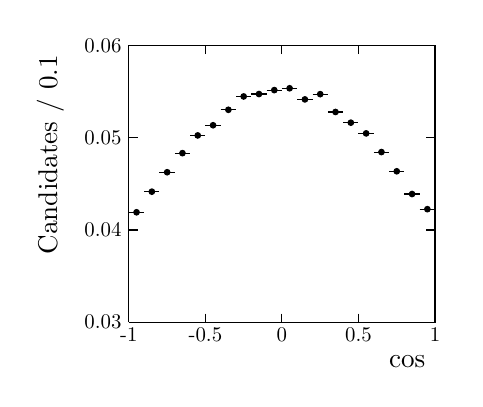
\begin{tikzpicture}
\pgfdeclareplotmark{cross} {
\pgfpathmoveto{\pgfpoint{-0.3\pgfplotmarksize}{\pgfplotmarksize}}
\pgfpathlineto{\pgfpoint{+0.3\pgfplotmarksize}{\pgfplotmarksize}}
\pgfpathlineto{\pgfpoint{+0.3\pgfplotmarksize}{0.3\pgfplotmarksize}}
\pgfpathlineto{\pgfpoint{+1\pgfplotmarksize}{0.3\pgfplotmarksize}}
\pgfpathlineto{\pgfpoint{+1\pgfplotmarksize}{-0.3\pgfplotmarksize}}
\pgfpathlineto{\pgfpoint{+0.3\pgfplotmarksize}{-0.3\pgfplotmarksize}}
\pgfpathlineto{\pgfpoint{+0.3\pgfplotmarksize}{-1.\pgfplotmarksize}}
\pgfpathlineto{\pgfpoint{-0.3\pgfplotmarksize}{-1.\pgfplotmarksize}}
\pgfpathlineto{\pgfpoint{-0.3\pgfplotmarksize}{-0.3\pgfplotmarksize}}
\pgfpathlineto{\pgfpoint{-1.\pgfplotmarksize}{-0.3\pgfplotmarksize}}
\pgfpathlineto{\pgfpoint{-1.\pgfplotmarksize}{0.3\pgfplotmarksize}}
\pgfpathlineto{\pgfpoint{-0.3\pgfplotmarksize}{0.3\pgfplotmarksize}}
\pgfpathclose
\pgfusepathqstroke
}
\pgfdeclareplotmark{cross*} {
\pgfpathmoveto{\pgfpoint{-0.3\pgfplotmarksize}{\pgfplotmarksize}}
\pgfpathlineto{\pgfpoint{+0.3\pgfplotmarksize}{\pgfplotmarksize}}
\pgfpathlineto{\pgfpoint{+0.3\pgfplotmarksize}{0.3\pgfplotmarksize}}
\pgfpathlineto{\pgfpoint{+1\pgfplotmarksize}{0.3\pgfplotmarksize}}
\pgfpathlineto{\pgfpoint{+1\pgfplotmarksize}{-0.3\pgfplotmarksize}}
\pgfpathlineto{\pgfpoint{+0.3\pgfplotmarksize}{-0.3\pgfplotmarksize}}
\pgfpathlineto{\pgfpoint{+0.3\pgfplotmarksize}{-1.\pgfplotmarksize}}
\pgfpathlineto{\pgfpoint{-0.3\pgfplotmarksize}{-1.\pgfplotmarksize}}
\pgfpathlineto{\pgfpoint{-0.3\pgfplotmarksize}{-0.3\pgfplotmarksize}}
\pgfpathlineto{\pgfpoint{-1.\pgfplotmarksize}{-0.3\pgfplotmarksize}}
\pgfpathlineto{\pgfpoint{-1.\pgfplotmarksize}{0.3\pgfplotmarksize}}
\pgfpathlineto{\pgfpoint{-0.3\pgfplotmarksize}{0.3\pgfplotmarksize}}
\pgfpathclose
\pgfusepathqfillstroke
}
\pgfdeclareplotmark{newstar} {
\pgfpathmoveto{\pgfqpoint{0pt}{\pgfplotmarksize}}
\pgfpathlineto{\pgfqpointpolar{44}{0.5\pgfplotmarksize}}
\pgfpathlineto{\pgfqpointpolar{18}{\pgfplotmarksize}}
\pgfpathlineto{\pgfqpointpolar{-20}{0.5\pgfplotmarksize}}
\pgfpathlineto{\pgfqpointpolar{-54}{\pgfplotmarksize}}
\pgfpathlineto{\pgfqpointpolar{-90}{0.5\pgfplotmarksize}}
\pgfpathlineto{\pgfqpointpolar{234}{\pgfplotmarksize}}
\pgfpathlineto{\pgfqpointpolar{198}{0.5\pgfplotmarksize}}
\pgfpathlineto{\pgfqpointpolar{162}{\pgfplotmarksize}}
\pgfpathlineto{\pgfqpointpolar{134}{0.5\pgfplotmarksize}}
\pgfpathclose
\pgfusepathqstroke
}
\pgfdeclareplotmark{newstar*} {
\pgfpathmoveto{\pgfqpoint{0pt}{\pgfplotmarksize}}
\pgfpathlineto{\pgfqpointpolar{44}{0.5\pgfplotmarksize}}
\pgfpathlineto{\pgfqpointpolar{18}{\pgfplotmarksize}}
\pgfpathlineto{\pgfqpointpolar{-20}{0.5\pgfplotmarksize}}
\pgfpathlineto{\pgfqpointpolar{-54}{\pgfplotmarksize}}
\pgfpathlineto{\pgfqpointpolar{-90}{0.5\pgfplotmarksize}}
\pgfpathlineto{\pgfqpointpolar{234}{\pgfplotmarksize}}
\pgfpathlineto{\pgfqpointpolar{198}{0.5\pgfplotmarksize}}
\pgfpathlineto{\pgfqpointpolar{162}{\pgfplotmarksize}}
\pgfpathlineto{\pgfqpointpolar{134}{0.5\pgfplotmarksize}}
\pgfpathclose
\pgfusepathqfillstroke
}
\definecolor{c}{rgb}{1,1,1};
\draw [color=c, fill=c] (0.1,4.72095) rectangle (4.9,9.16419);
\draw [color=c, fill=c] (0.772,5.43186) rectangle (4.66,8.94203);
\definecolor{c}{rgb}{0,0,0};
\draw [c] (0.772,5.43186) -- (0.772,8.94203) -- (4.66,8.94203) -- (4.66,5.43186) -- (0.772,5.43186);
\draw [c,line width=0.4] (0.8692,6.8025) -- (0.8692,6.82645);
\draw [c,line width=0.4] (0.8692,6.82645) -- (0.8692,6.85041);
\draw [c,line width=0.4] (0.772,6.82645) -- (0.8692,6.82645);
\draw [c,line width=0.4] (0.8692,6.82645) -- (0.9664,6.82645);
\foreach \P in {(0.8692,6.82645)}{\draw[mark options={color=c,fill=c},mark size=1.201201pt,mark=*,mark size=1pt] plot coordinates {\P};}
\draw [c,line width=0.4] (1.0636,7.06372) -- (1.0636,7.08831);
\draw [c,line width=0.4] (1.0636,7.08831) -- (1.0636,7.1129);
\draw [c,line width=0.4] (0.9664,7.08831) -- (1.0636,7.08831);
\draw [c,line width=0.4] (1.0636,7.08831) -- (1.1608,7.08831);
\foreach \P in {(1.0636,7.08831)}{\draw[mark options={color=c,fill=c},mark size=1.201201pt,mark=*,mark size=1pt] plot coordinates {\P};}
\draw [c,line width=0.4] (1.258,7.31002) -- (1.258,7.33519);
\draw [c,line width=0.4] (1.258,7.33519) -- (1.258,7.36036);
\draw [c,line width=0.4] (1.1608,7.33519) -- (1.258,7.33519);
\draw [c,line width=0.4] (1.258,7.33519) -- (1.3552,7.33519);
\foreach \P in {(1.258,7.33519)}{\draw[mark options={color=c,fill=c},mark size=1.201201pt,mark=*,mark size=1pt] plot coordinates {\P};}
\draw [c,line width=0.4] (1.4524,7.55202) -- (1.4524,7.57774);
\draw [c,line width=0.4] (1.4524,7.57774) -- (1.4524,7.60347);
\draw [c,line width=0.4] (1.3552,7.57774) -- (1.4524,7.57774);
\draw [c,line width=0.4] (1.4524,7.57774) -- (1.5496,7.57774);
\foreach \P in {(1.4524,7.57774)}{\draw[mark options={color=c,fill=c},mark size=1.201201pt,mark=*,mark size=1pt] plot coordinates {\P};}
\draw [c,line width=0.4] (1.6468,7.7764) -- (1.6468,7.80263);
\draw [c,line width=0.4] (1.6468,7.80263) -- (1.6468,7.82886);
\draw [c,line width=0.4] (1.5496,7.80263) -- (1.6468,7.80263);
\draw [c,line width=0.4] (1.6468,7.80263) -- (1.744,7.80263);
\foreach \P in {(1.6468,7.80263)}{\draw[mark options={color=c,fill=c},mark size=1.201201pt,mark=*,mark size=1pt] plot coordinates {\P};}
\draw [c,line width=0.4] (1.8412,7.9054) -- (1.8412,7.93192);
\draw [c,line width=0.4] (1.8412,7.93192) -- (1.8412,7.95844);
\draw [c,line width=0.4] (1.744,7.93192) -- (1.8412,7.93192);
\draw [c,line width=0.4] (1.8412,7.93192) -- (1.9384,7.93192);
\foreach \P in {(1.8412,7.93192)}{\draw[mark options={color=c,fill=c},mark size=1.201201pt,mark=*,mark size=1pt] plot coordinates {\P};}
\draw [c,line width=0.4] (2.0356,8.10119) -- (2.0356,8.12814);
\draw [c,line width=0.4] (2.0356,8.12814) -- (2.0356,8.15509);
\draw [c,line width=0.4] (1.9384,8.12814) -- (2.0356,8.12814);
\draw [c,line width=0.4] (2.0356,8.12814) -- (2.1328,8.12814);
\foreach \P in {(2.0356,8.12814)}{\draw[mark options={color=c,fill=c},mark size=1.201201pt,mark=*,mark size=1pt] plot coordinates {\P};}
\draw [c,line width=0.4] (2.23,8.27025) -- (2.23,8.29756);
\draw [c,line width=0.4] (2.23,8.29756) -- (2.23,8.32487);
\draw [c,line width=0.4] (2.1328,8.29756) -- (2.23,8.29756);
\draw [c,line width=0.4] (2.23,8.29756) -- (2.3272,8.29756);
\foreach \P in {(2.23,8.29756)}{\draw[mark options={color=c,fill=c},mark size=1.201201pt,mark=*,mark size=1pt] plot coordinates {\P};}
\draw [c,line width=0.4] (2.4244,8.30084) -- (2.4244,8.32822);
\draw [c,line width=0.4] (2.4244,8.32822) -- (2.4244,8.3556);
\draw [c,line width=0.4] (2.3272,8.32822) -- (2.4244,8.32822);
\draw [c,line width=0.4] (2.4244,8.32822) -- (2.5216,8.32822);
\foreach \P in {(2.4244,8.32822)}{\draw[mark options={color=c,fill=c},mark size=1.201201pt,mark=*,mark size=1pt] plot coordinates {\P};}
\draw [c,line width=0.4] (2.6188,8.35069) -- (2.6188,8.37818);
\draw [c,line width=0.4] (2.6188,8.37818) -- (2.6188,8.40566);
\draw [c,line width=0.4] (2.5216,8.37818) -- (2.6188,8.37818);
\draw [c,line width=0.4] (2.6188,8.37818) -- (2.716,8.37818);
\foreach \P in {(2.6188,8.37818)}{\draw[mark options={color=c,fill=c},mark size=1.201201pt,mark=*,mark size=1pt] plot coordinates {\P};}
\draw [c,line width=0.4] (2.8132,8.37404) -- (2.8132,8.40158);
\draw [c,line width=0.4] (2.8132,8.40158) -- (2.8132,8.42911);
\draw [c,line width=0.4] (2.716,8.40158) -- (2.8132,8.40158);
\draw [c,line width=0.4] (2.8132,8.40158) -- (2.9104,8.40158);
\foreach \P in {(2.8132,8.40158)}{\draw[mark options={color=c,fill=c},mark size=1.201201pt,mark=*,mark size=1pt] plot coordinates {\P};}
\draw [c,line width=0.4] (3.0076,8.233) -- (3.0076,8.26024);
\draw [c,line width=0.4] (3.0076,8.26024) -- (3.0076,8.28747);
\draw [c,line width=0.4] (2.9104,8.26024) -- (3.0076,8.26024);
\draw [c,line width=0.4] (3.0076,8.26024) -- (3.1048,8.26024);
\foreach \P in {(3.0076,8.26024)}{\draw[mark options={color=c,fill=c},mark size=1.201201pt,mark=*,mark size=1pt] plot coordinates {\P};}
\draw [c,line width=0.4] (3.202,8.29944) -- (3.202,8.32681);
\draw [c,line width=0.4] (3.202,8.32681) -- (3.202,8.35419);
\draw [c,line width=0.4] (3.1048,8.32681) -- (3.202,8.32681);
\draw [c,line width=0.4] (3.202,8.32681) -- (3.2992,8.32681);
\foreach \P in {(3.202,8.32681)}{\draw[mark options={color=c,fill=c},mark size=1.201201pt,mark=*,mark size=1pt] plot coordinates {\P};}
\draw [c,line width=0.4] (3.3964,8.07364) -- (3.3964,8.10052);
\draw [c,line width=0.4] (3.3964,8.10052) -- (3.3964,8.12741);
\draw [c,line width=0.4] (3.2992,8.10052) -- (3.3964,8.10052);
\draw [c,line width=0.4] (3.3964,8.10052) -- (3.4936,8.10052);
\foreach \P in {(3.3964,8.10052)}{\draw[mark options={color=c,fill=c},mark size=1.201201pt,mark=*,mark size=1pt] plot coordinates {\P};}
\draw [c,line width=0.4] (3.5908,7.93797) -- (3.5908,7.96456);
\draw [c,line width=0.4] (3.5908,7.96456) -- (3.5908,7.99115);
\draw [c,line width=0.4] (3.4936,7.96456) -- (3.5908,7.96456);
\draw [c,line width=0.4] (3.5908,7.96456) -- (3.688,7.96456);
\foreach \P in {(3.5908,7.96456)}{\draw[mark options={color=c,fill=c},mark size=1.201201pt,mark=*,mark size=1pt] plot coordinates {\P};}
\draw [c,line width=0.4] (3.7852,7.8022) -- (3.7852,7.82849);
\draw [c,line width=0.4] (3.7852,7.82849) -- (3.7852,7.85478);
\draw [c,line width=0.4] (3.688,7.82849) -- (3.7852,7.82849);
\draw [c,line width=0.4] (3.7852,7.82849) -- (3.8824,7.82849);
\foreach \P in {(3.7852,7.82849)}{\draw[mark options={color=c,fill=c},mark size=1.201201pt,mark=*,mark size=1pt] plot coordinates {\P};}
\draw [c,line width=0.4] (3.9796,7.56556) -- (3.9796,7.59132);
\draw [c,line width=0.4] (3.9796,7.59132) -- (3.9796,7.61707);
\draw [c,line width=0.4] (3.8824,7.59132) -- (3.9796,7.59132);
\draw [c,line width=0.4] (3.9796,7.59132) -- (4.0768,7.59132);
\foreach \P in {(3.9796,7.59132)}{\draw[mark options={color=c,fill=c},mark size=1.201201pt,mark=*,mark size=1pt] plot coordinates {\P};}
\draw [c,line width=0.4] (4.174,7.32193) -- (4.174,7.34713);
\draw [c,line width=0.4] (4.174,7.34713) -- (4.174,7.37232);
\draw [c,line width=0.4] (4.0768,7.34713) -- (4.174,7.34713);
\draw [c,line width=0.4] (4.174,7.34713) -- (4.2712,7.34713);
\foreach \P in {(4.174,7.34713)}{\draw[mark options={color=c,fill=c},mark size=1.201201pt,mark=*,mark size=1pt] plot coordinates {\P};}
\draw [c,line width=0.4] (4.3684,7.03396) -- (4.3684,7.05847);
\draw [c,line width=0.4] (4.3684,7.05847) -- (4.3684,7.08299);
\draw [c,line width=0.4] (4.2712,7.05847) -- (4.3684,7.05847);
\draw [c,line width=0.4] (4.3684,7.05847) -- (4.4656,7.05847);
\foreach \P in {(4.3684,7.05847)}{\draw[mark options={color=c,fill=c},mark size=1.201201pt,mark=*,mark size=1pt] plot coordinates {\P};}
\draw [c,line width=0.4] (4.5628,6.84195) -- (4.5628,6.866);
\draw [c,line width=0.4] (4.5628,6.866) -- (4.5628,6.89005);
\draw [c,line width=0.4] (4.4656,6.866) -- (4.5628,6.866);
\draw [c,line width=0.4] (4.5628,6.866) -- (4.66,6.866);
\foreach \P in {(4.5628,6.866)}{\draw[mark options={color=c,fill=c},mark size=1.201201pt,mark=*,mark size=1pt] plot coordinates {\P};}
\draw [c,line width=0.4] (0.772,5.43186) -- (4.66,5.43186);
\draw [anchor= east] (4.66,4.93422) node[scale=0.979298, rotate=0]{$\cos\thetamu$};
\draw [c,line width=0.4] (0.772,5.53984) -- (0.772,5.43186);
\draw [c,line width=0.4] (1.744,5.53984) -- (1.744,5.43186);
\draw [c,line width=0.4] (2.716,5.53984) -- (2.716,5.43186);
\draw [c,line width=0.4] (3.688,5.53984) -- (3.688,5.43186);
\draw [c,line width=0.4] (4.66,5.53984) -- (4.66,5.43186);
\draw [anchor=base] (0.772,5.19193) node[scale=0.753306, rotate=0]{-1};
\draw [anchor=base] (1.744,5.19193) node[scale=0.753306, rotate=0]{-0.5};
\draw [anchor=base] (2.716,5.19193) node[scale=0.753306, rotate=0]{0};
\draw [anchor=base] (3.688,5.19193) node[scale=0.753306, rotate=0]{0.5};
\draw [anchor=base] (4.66,5.19193) node[scale=0.753306, rotate=0]{1};
\draw [c,line width=0.4] (0.772,8.94203) -- (4.66,8.94203);
\draw [c,line width=0.4] (0.772,8.83406) -- (0.772,8.94203);
\draw [c,line width=0.4] (1.744,8.83406) -- (1.744,8.94203);
\draw [c,line width=0.4] (2.716,8.83406) -- (2.716,8.94203);
\draw [c,line width=0.4] (3.688,8.83406) -- (3.688,8.94203);
\draw [c,line width=0.4] (4.66,8.83406) -- (4.66,8.94203);
\draw [c,line width=0.4] (0.772,5.43186) -- (0.772,8.94203);
\draw [anchor= east] (-0.2264,8.94203) node[scale=0.979298, rotate=90]{Candidates / 0.1};
\draw [c,line width=0.4] (0.88576,5.43186) -- (0.772,5.43186);
\draw [c,line width=0.4] (0.88576,6.60192) -- (0.772,6.60192);
\draw [c,line width=0.4] (0.88576,7.77197) -- (0.772,7.77197);
\draw [c,line width=0.4] (0.88576,8.94203) -- (0.772,8.94203);
\draw [c,line width=0.4] (0.88576,8.94203) -- (0.772,8.94203);
\draw [anchor= east] (0.772,5.43186) node[scale=0.753306, rotate=0]{0.03};
\draw [anchor= east] (0.772,6.60192) node[scale=0.753306, rotate=0]{0.04};
\draw [anchor= east] (0.772,7.77197) node[scale=0.753306, rotate=0]{0.05};
\draw [anchor= east] (0.772,8.94203) node[scale=0.753306, rotate=0]{0.06};
\draw [c,line width=0.4] (4.66,5.43186) -- (4.66,8.94203);
\draw [c,line width=0.4] (4.54624,5.43186) -- (4.66,5.43186);
\draw [c,line width=0.4] (4.54624,6.60192) -- (4.66,6.60192);
\draw [c,line width=0.4] (4.54624,7.77197) -- (4.66,7.77197);
\draw [c,line width=0.4] (4.54624,8.94203) -- (4.66,8.94203);
\draw [c,line width=0.4] (4.54624,8.94203) -- (4.66,8.94203);
\end{tikzpicture}
